Consider a simple, non-empty Graph $G = (V, E)$ comprising a set of Edges $E$ and vertices $E$.
For specificity, $E(G)$ and $V(G)$ is used to refer to the set of edges and vertices associated
with Graph $G$ respectively, where required.Further, denote by $|V|$ the cardinality of set of
vertices $V$, let $G$ be a Graph with $|V(G)| = |\{v_1, v_2, \ldots, v_n \}| = n$ vertices and
$|E(G)| = m$ edges with $E \subset \binom{V}{2} $;
where $\binom{V}{2} = \left\{\left\langle u,v\right\rangle | u,v \in V, u \neq v \right\} $, that is,
the set of all possible unordered pairs created from $V$. For each $e = \left\langle u, v\right\rangle \in E$,
$e$ is said to be incident on $u,v\in V$, whereas $u$ and $v$ are adjacent to each other.

The Neighbor set $\mathcal{N}(v)$ of $v \in V$, defined as
$\mathcal{N}(v) =: \left\{w  \in V(G) | v \neq w, \exists e \in E(G)\right\} $  is the set of vertices
(other than $v$) adjacent to $v \tilde{\mathcal{V}}  \bar{\mathcal{V}}$. Given a Graph $\mathcal{G}$,
$\mathcal{G} \subseteq G$ denotes that $\mathcal{G}$ is a subgraph of $G$, if it holds that
$\forall e \in E(\mathcal{G}),  \; u,v \subseteq V(\mathcal{G})$, $V(\mathcal{G}) \subseteq V(G)$
and $E(\mathcal{G}) \subseteq E(G)$.

The adjacency matrix of a weighted graph $G$ is a symmetric matrix $A \in \mathbb{R}^{n \times n}$ with $i$th row and $j$th
column containing the number of edges incident on vertex $v_i$ and $v_j$. More precisely,
let $\omega : \left\{ 0,1 \right\} \mapsto \mathbb{R}^+_0$ for $i,j \in \left\{1,2, \ldots, n \right\} $

\begin{equation}\label{eqn: adj_matrix}
  A_{i,j} = \begin{cases}
    \omega (e_i), & \qquad e_i = \left\langle v_i, v_j\right\rangle \in E(G) \\
    0,            & \qquad \text{otherwise.}
  \end{cases}
\end{equation}
By restricting \eqref{eqn: adj_matrix} $\omega \in \left\{ 0,1 \right\} \;\forall  \omega  (e_i), \; e_i  \in E$, we recover the
adjacency matrix of an unweighted graph. The volume $vol(F)$ of a a subset of nodes $F \in V$ is the sum of weight of edges adjacent
to the nodes of $F$ and given as $vol(F) = \sum_{v_i \in F}  \delta(v_i)$; where $\delta(v_i)$ is the degree of vertex $v_i$ obtained
as the sum of the weights of edges incident on it: $\delta(v_i) = \sum_{i = 1}^{n} A_{i,j} $.

Denote the number of components in of graph $G$ by $\kappa(G)$. For the a set $V^* \subseteq V(G)$, $V^*$ is a cut-vertex
if $\kappa(G[V(G)\backslash V^* = \tilde{V} ]) > \kappa(G)$; where  $G[\tilde{V}]$ is the graph induced by $\tilde{V}$

\begin{question}[Node Selection]
  \label{pythagorean}
  Is it possible to ensure that the selection of critical nodes in the network is based on both articulation points and their respective changing weights?
  (Where the weight on each critical (or cut) node is the total amount of traffic load generated from non-articulation points).
\end{question}

\begin{approach}
  We would have two optimization objectives base on:
  \begin{enumerate}
    \item maximum volume
    \item cut vertices.
  \end{enumerate}
\end{approach}


\begin{problem}
Given a Graph $G = (V, E)$, let $ \tilde{V} = V(G)\backslash V^*$. Denote by $\vartheta (G)$ the set of cut-vertices associated with Graph $G$ defined by
\begin{equation}
  \vartheta (G) =\left\{(v_i, v_j)\in V^* \; \vert \; \kappa(G[\tilde{V} ]) > \kappa(G)\right\}.
\end{equation}
Further, let the set $\vartheta (\tilde{G} )$ partition  $\vartheta (G)$, that is,
$\vartheta (\tilde{G}) = \bigcup_{i=1}^n \vartheta (G_i)$ where each  $\vartheta (G_i)$ represents each
vertex-cut associated with $\vartheta (G)$. The traffic on $\vartheta (G_i)$ is represented by its volume
of edges $e \in E(G)$
incident on it and expressed as
\begin{equation}
  vol(\vartheta (G_i)) = \sum_{\vartheta (G_i)\in G} \delta(\vartheta (G_i))
\end{equation}

\end{problem}

\begin{figure}[htb!]
  \centering 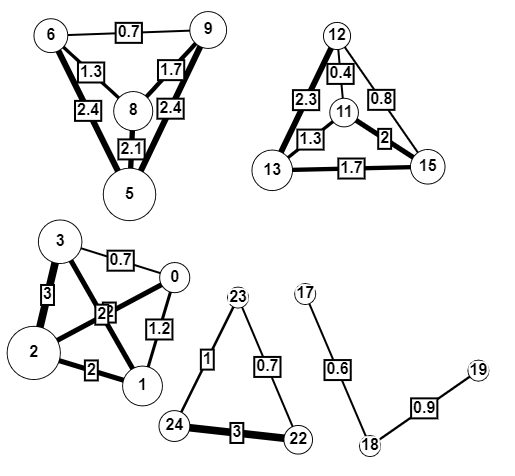
\includegraphics[width=\textwidth]{figures/cut_sample_2.png}
  \caption{Cut Vertices}
  \label{fig:cdnp}
\end{figure}